\documentclass[10pt,letterpaper,onecolumn]{article}
\usepackage[latin1]{inputenc}
\usepackage{amsmath}
\usepackage{amsfonts}
\usepackage{amssymb}
\usepackage{graphicx}
\usepackage{booktabs}
\usepackage{color}
\usepackage{array}
\usepackage[left=1in, right=1in, top=1in, bottom=1in]{geometry}
\author{Sukanya Sharma}
\title{\vspace*{-1cm}
  Impact of Short Term Rentals on the Rental Affordability in San Fransisco \\{\large\textsc{The Case of Airbnb}}}
\date{\emph{Defended:} June, 2018}
\usepackage{url}
\usepackage{float}
\usepackage{tikz}
\usetikzlibrary{shapes.geometric, arrows}
\usepackage[hidelinks]{hyperref}

\begin{document}
\maketitle

\noindent Submitted in partial fulfillment of the requirements for the degree of Master of Urban Planning 2018 at the University of Illinois at Urbana-Champaign.

\emph{Masters Committee:}
Associate Professor Bumsoo Lee (advisor),
Assistant Professor Andrew Greenlee

\abstract{
Short term rentals listed on Airbnb and like platforms are common place all over the world. The advent of Airbnb operating on sharing economy models is a global phenomenon. Policy debates have naturally followed. Gauging impacts of such platforms is crucial and potentially can inform policy. Airbnb rentals all over the world, questions have been raised about their impacts (Meni, 2017). While one side discusses the democratization of tourism industry and how Airbnb makes it easier for tourists to travel and experience places, the other side brings forth the skirting of hotel taxes and negative neighborhood externalities that inevitably result from these rentals. Airbnb has attracted controversy in cities all over the world, with high-profile lawsuits centered around criticism for evasion of taxes and for avoiding regulatory oversight that is otherwise enforced on hotels and providers of similar services. The presented paper is an attempt to gauge the impact of Airbnb on rental affordability by using spatial econometric analyses. The study areas for the aforementioned research is the San Francisco Metropolitan Statistical Area (SF MSA).

The hypothesis is that an increase in the Airbnb listings (i.e. the short-term housing stock) in the study area is correlated negatively with rental affordability, causing it to decrease. Key research questions are does Airbnb impact the rental affordability in an area? If yes, then, to what extent? To answer these questions, both cross-sectional and longitudinal analyses are undertaken. Aiming to contribute to the body of literature, revolving around the debate through quantitative analyses and regulatory policy discussion, this study finds positive and statistically significant correlation between both Airbnb variables (percent Airbnb listings as a proportion of rental housing units and weighted Airbnb listings based on listing types) and variables representing rental affordability like percent rent-burdened and overburdened households, median rents and median house prices). Various models were considered for both cross-sectional and longitudinal analyses using different combinations of the aforementioned variables. The spatial econometric analysis answers one of our key questions in the affirmative -- the presence of Airbnb rentals does impact the rental affordability in an area.

Having established a relationship, our second objective was to gauge this impact's extent. Simulations were run to understand the results of the spatial econometrics models to help visualize this impact. In the case of cross-sectional analysis for San Francisco MSA, these simulations showed that for a typical census tract (one with median percentage of Airbnb listings, as a fraction of the rental housing market) a 1\% increase in Airbnb listings corresponded to a 0.06\% rise in the rent overburdened household category. Hence, in the case of a census tract with 10,000 households, a 10\% increase in percent Airbnb listings will correspond to 60 more households being added to the rent overburdened category.
This effect is more pronounced for tracts with a lower number of Airbnb listings (10th or 25th percentiles). Additionally, tracts with no or a low percentage of Airbnb listings will have more households pushed to a rent-burdened category, with a similar rise in Airbnb listings. 

In the case of longitudinal analysis of panel data for San Francisco City for a period of four years (2013-- 2016), the simulations show that census tracts with a smaller presence of Airbnb listings (those below the 50th percentile) were more sensitive to an increase in Airbnb listings i.e. they saw a higher increase in the median house price per tract as compared to census tracts in the higher percentiles. This trend was consistent across all four years affirming the extent of the impact of Airbnb listings on the rental affordability in an area.}


\section*{Chapter 1: Introduction}\label{sec: introduction}

A major motivation for this research is the acute housing affordability
crisis in US. California, like many other states currently faces a
housing affordability crisis, the effects of which are particularly
strong in the bay area. San Francisco city and MSA (including counties
Alameda, Contra Costa, San Francisco, Marin and San Mateo) continue to
show drops in rental as well as housing affordability levels. With the
affordability situation this dire, a decrease in housing stock poses a
major threat. In the case of rental affordability, the decrease in
long-term rentals can lead to further increase in rent and consequently
a decrease in rental affordability. This makes a case for this research
and is one of the main motivations for this study.

Platforms like Airbnb are redefining tourist consumption patterns in
ways that can impact housing affordability. From humble beginnings as a
start-up in San Francisco in 2008, the platform is now valued at over 31
billion dollars\footnote{Bensinger, Greg. Airbnb Valued at \$31 Billion
  After New Funding Round; Home-sharing site adds \$1 billion cash
  cushion to stave off IPO, Wall Street Journal (Online); New York, N.Y.
  09 Mar 2017. Retrieved from:
  \url{https://www.wsj.com/articles/airbnb-valued-at-31-billion-after-new-funding-round-1489086240}},
is present in 190 countries worldwide, while continuing to operate on
the principles of sharing economy, peer-to-peer markets and the
`digital' economy. Airbnb and like platforms reaching such high
valuations and becoming commonplace, it has become imperative to
critically gauge their impacts.

There is an emerging body of literature investigating the relationship
between Airbnb and housing related outcomes, such as average rent,
tourism, rates of hotel usage, and more. These studies vary widely in
their methods and represent a new field of study within housing policy
and urban planning, some of which are discussed in the literature review
of this research. The debate is divisive, and analysts is divided
firstly on whether Airbnb has any effect at all and secondly whether
these effects are positive or negative.

The presented research is an inquiry into the impacts of short-term
rentals on the rent affordability of the study area. Due to the largest
share among its competitors and its popularity, this study chose Airbnb
as a representative platform for short-term rentals. One of the main
motivations of this research is the affordability crisis afflicting most
cities in the US and particularly San Francisco. This research finds its
roots in understanding the complex dynamics of having Airbnb like
platforms in an area which is undergoing a worsening affordability
crisis. Additionally, this study aims to contribute to the discourse of
one of the most pressing question -- regulating sharing economy by
adding data to the debate. The following section elaborates on the
hypothesis, aims and methodology undertaken of this research.

\subsection*{1.1 Hypothesis}\label{subsec: hypothesis}

This research uses spatial econometrics techniques to examine the impact
of Airbnb on the rental affordability and long-term rental housing stock
in the San Francisco MSA. It hypothesizes is that with an increase in
the Airbnb listings (i.e. short-term rental housing stock) there is a
decrease in the rental affordability in the study area. This is studied
using various locational, socio-economic and neighborhood level
variables. More formally, the hypothesis states that the variables log
percent Airbnb rentals (active and all rentals) and weighted Airbnb
listings are significantly and positively correlated to rental
affordability measures and rents (rent burdened, rent overburdened and
gross median rent). Key research questions are \emph{does Airbnb impact
rental affordability in an area? If yes, then to what extent?}

\subsection*{1.2 Objectives and Methodology}\label{objectives-and-methodology}
The objectives of this research are as follows:

\begin{itemize}
\item
  To study the impacts of short-term rentals in the form of Airbnb
  listings on the rental affordability in the San Francisco Metropolitan
  Statistical Area (MSA) and San Francisco City.
\item
  To undertake a policy discussion on possible regulatory response to
  Airbnb and like platforms and sharing economy in general.
\end{itemize}

\begin{figure}[H]
  \centering
  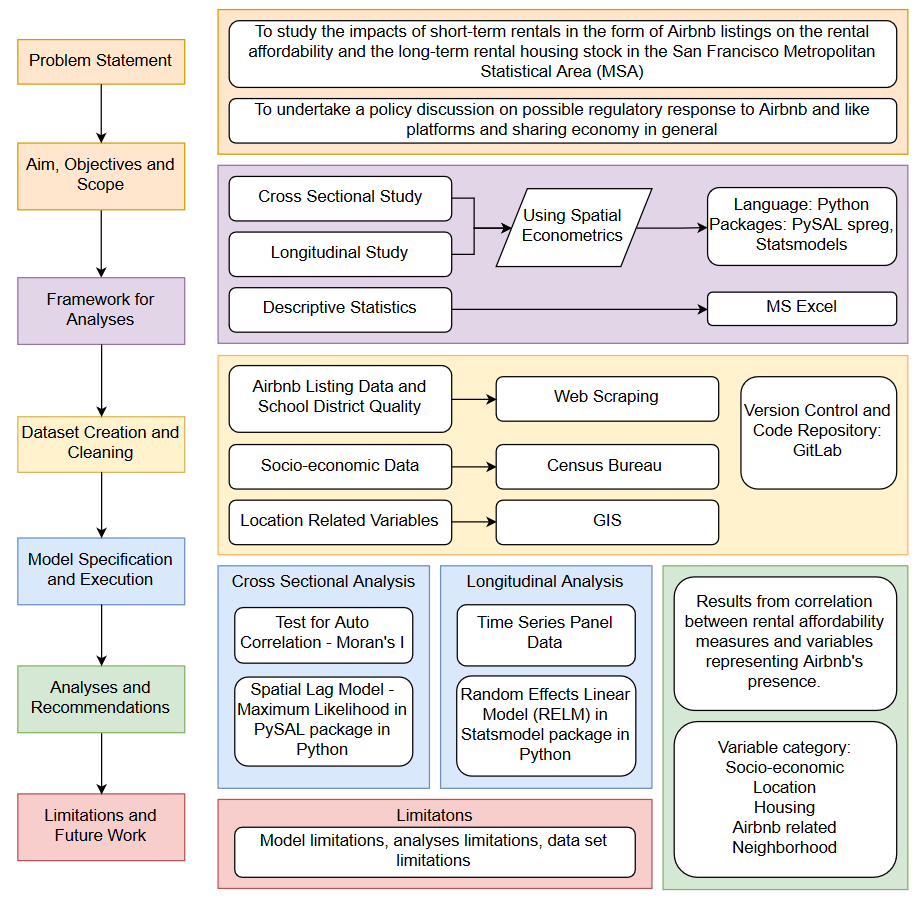
\includegraphics[width=0.8\textwidth]{Research_Methodology.png}
  \\{\hfill\scriptsize Source: author.\hspace{1.3cm}}
  \caption{Research methodology.}
\end{figure}

For the purposes of this research, both cross-sectional and longitudinal
research was conducted. The research methodology presented in the figure
above shows the steps that were undertaken and details of those steps.
As shown in the figure, analyses were divided into two main
sections---the cross-sectional analysis and longitudinal. A detailed
treatment of these analyses is carried out in Chapters 3 and 4.


%%%%%%%%%%%%%%%%%%%%%%%%%%%%%%%%%%%%%%%%%%%%%%%%%%%%%%%%%%%%%%%%%%%%%%%%%%%%%%%
\section*{Chapter 3: Data and Methods}
%%%%%%%%%%%%%%%%%%%%%%%%%%%%%%%%%%%%%%%%%%%%%%%%%%%%%%%%%%%%%%%%%%%%%%%%%%%%%%

As mentioned in the chapter 1, this study conducts both cross-sectional
and longitudinal analysis. This chapter details out the methods used,
the theory behind those methods, dataset generation, our unit of
analysis and the variables considered. It is important to note here that
the cross-sectional analysis was carried out for the San Francisco MSA
(a five-county region) whereas the longitudinal analysis was carried out
for San Francisco city due to limited availability of data on Airbnb
listings.

{\color{red} \emph{Note: The section on Longitudinal Analysis has been omitted from this extract for the sake of brevity.}}

\subsection*{3.1 Cross-sectional Analysis}

The cross-sectional analysis was carried out to provide information on
the characteristics of and statistical relationships between selected
dependent and independent variables, at a specific moment in time --
2017 for this research.

\subsubsection*{Study Area}

The chosen area for the cross-sectional study was the San
Francisco-Oakland-Hayward MSA (Metropolitan Statistical Area) which is a
five-county region in California with a population of 4,679,166 (2016
ACS estimate) and an area of 2,474 square miles (6,410 km\(^2\)). It consists
of Alameda County, Contra Costa County, San Francisco County, San Mateo
County, and Marin County. To better gauge the extent of spatial
correlation and expand the analysis, the MSA area was selected so as to
not confine the analysis to San Francisco City. This five-county area
includes major urban centers as well as suburban development and few
rural areas. This diversity also helped in understanding the impact of
Airbnb listings beyond just a city/urban area. Figure~2 shows the
five-county study region and Airbnb listings in it.

\begin{figure}[H]
  \centering
  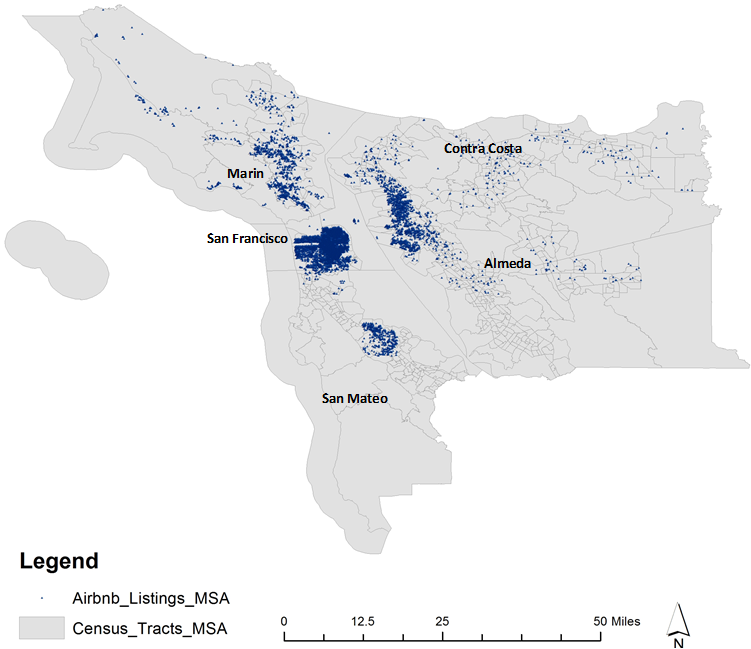
\includegraphics[width=0.6\textwidth]{Airbnb_listings.png}
  \caption{Airbnb listings in San Francisco MSA as of 2017.}
\end{figure}


\subsection*{3.2 Dataset Generation}

For the purposes of dataset creation, various methods were used to
collect relevant data. For the Airbnb listing data, a script\footnote{Available
at GitLab
(\url{https://gitlab-beta.engr.illinois.edu/sukanya3/Airbnb_Spatial_Econometrics})
under open license} was developed in Python using selenium and
PostgreSQL packages to scrape data off of airbnb.com. The scraping was
undertaken for all five counties in the study area and listings data was
extracted with their location coordinates using the bounding box method.
The scraping was undertaken in December 2017. In addition to using
Airbnb listings as a percentage of rental housing units\footnote{Rental
housing data obtained from 2016 ACS estimates}, a composite score
index was created which incorporated the difference of listing type. A
weight of 1 was given to entire house listings, 0.5 for private rooms
and 0.2 for shared rooms/couches etc. The distribution of percent Airbnb
listing and weighted listings indicate positively skewed distributions
as shown in the figure below. Hence to account for heteroskedasticity,
all variables used in the model are natural logarithms (except the dummy
variable) were log-transformed.

\begin{figure}[H]
  \centering
  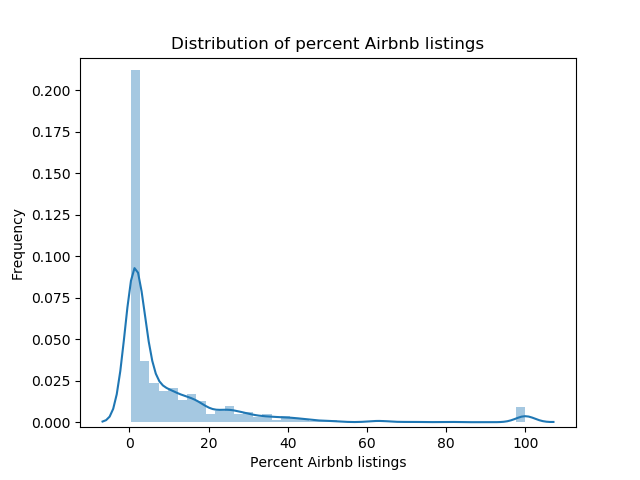
\includegraphics[width=0.49\textwidth]{Airbnb_listings_distribution.png}
  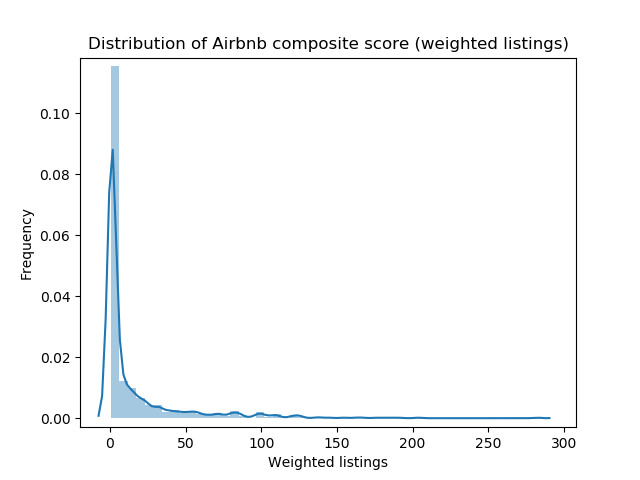
\includegraphics[width=0.49\textwidth]{Composite_score_distribution.png}
  \caption{Distribution of Airbnb listings in the study area}
\end{figure}

Data for independent (control) variables like \texttt{log percent unemployed population}, \texttt{log percent foreign-born population}, \texttt{log percent
non-white population}, \texttt{log rent burdened households} and \texttt{log rent
overburdened households} was obtained from the American Community
Survey, using 2016 estimates for the study area. This data was collected
at the census-tract level.

Another independent variable in the dataset is \texttt{log school district
quality} which is in the form of a score assigned by an independent
non-profit --- greatschools.org. The school quality is reflected from a
score called summary rating that the website gives based on various
criteria. According to the nonprofit, the summary rating is a
multi-measure school quality metric intended to reflect a school's
characteristics and quality across multiple dimensions, ultimately
representing the school's overall quality in preparing students for
postsecondary success. It is an aggregation of the school's
``sub-ratings'', which include test score, student progress, academic
progress, equity, college readiness, and advanced courses ratings, as
well as a flag for discipline and attendance issues\footnote{Methodology
used by Great Schools non-profit. Retrieved from
\url{https://www.greatschools.org/gk/ratings-methodology/}}. The data
for this variable was web-scraped from the greatschools.org website
using a Python script\footnote{Inspired by the script developed and
shared by Yongsung Lee, a Ph.D. candidate at School of City and
Regional Planning, Georgia Institute of Technology}.

The centroids of the census-tracts were used as address/locations for all schools in that
census-tract. The highest school quality score was selected in case of
multiple schools existing in the same tract. There was an element of
reverse geocoding the location coordinates of the census tract centroids
by using Google API to create addresses that the greatschools.org
website accepts for locating relevant schools at the high school level.

For the location variables like \texttt{Log BART dist} (log of Euclidian
distance of BART stations from census-tract centroid), \texttt{Coastline
tracts} (dummy variable where 1 denotes a coastline tract) and \texttt{Log
CBD dist} (log of Euclidian distance between nearest central business
district and centroid of the census-tract) were computed using ArcMap in
ArcGIS and its functions in ArcToolbox and network analyst.

For gauging job accessibility, two variables from the Smart Location
Database were used. The primary variables -- \texttt{D5ar} and \texttt{D5br} from the
destination accessibility dataset were used because they measure jobs or
working- age population within a 45-minute commute via automobile (\texttt{D5ar})
or transit (\texttt{D5br}). The ``r'' reflects the accessibility of job from
residences to jobs. This data was collected at the census-tract level
for all five counties in the study area. Table 1 shows the variable
categories and description in brief.

\begin{table}
\scriptsize
\def\arraystretch{1.5}
\begin{tabular}{>{\raggedright}p{3cm} >{\raggedright}p{3cm} >{\raggedright}p{3.5cm} >{\raggedright}p{3cm} >{\raggedright\arraybackslash}p{3cm}}
\toprule
\textbf{Variable \mbox{Category}}
  & \textbf{Variable Name}
  & \textbf{Description}
  & \textbf{Data Source}
  & \textbf{Remarks}\\
\midrule
\textbf{Independent Variables} & & & &\\
\midrule
\textbf{Airbnb}
  & Log Percent Airbnb
  & Log of Airbnb listings as a percentage of rental housing units
  & Airbnb.com web scrape and US Census TIGER/Line Files
  &\\
%
~ &Log Weighted Airbnb listings
  & Log of weighted Airbnb listings (1 for entire home, 0.5 for private room, 0.2 for shared room)
  & Airbnb.com web scrape
  &\\
%
\textbf{Location}
  & Log BART dist
  & Log Euclidean distance in meter between census tract centroid and nearest BART station
  & ArcMAP analysis and TIGER/Line shapefiles from Census Bureau
  &\\
%
~ & Log CBD dist
  & Log Euclidean distance in meter between census tract centroid and nearest Central Business District
  & ArcMAP analysis and TIGER/Line shapefiles from Census Bureau
  &\\
%
~ & Coastal tracts (Dummy)
  & if a census tract is at the coast line; otherwise 0
  & ArcMAP analysis and TIGER/Line shapefiles from Census Bureau
  &\\
%
\textbf{Demographic}
  & Log unemployment rate
  & Log of percentage unemployed people as a percentage of the civilian labor force
  & US Census TIGER/Line Files
  &\\
%
~ & Log percent non-white
  & Log of percentage population which is not white
  & US Census TIGER/Line Files
  &\\
%  
  & Log percent foreign-born
  & Log of percentage population who is not US citizen at birth, includes those who become US citizens through naturalization
  & US Census TIGER/Line Files
  &\\
%
\textbf{Neighborhood Level}
  & Log school district quality
  & Log of school district score as given by greatschools.org
  & Greatschool.org web scrape
  &\\
%
\textbf{Job Accessibility}
  & Log accessibility by car
  & Log of jobs within 45 minutes auto/car travel time; time-decay (network travel time) weighted
  & Smart Location Database, US EPA Smart Growth Program
  &\\
%
  & Log accessibility by transit
  & Jobs within 45-minute transit commute, distance decay (walk network travel time) weighted
  & Smart Location Database, US EPA Smart Growth Program
  &\\
%
\midrule
\textbf{Dependent Variable} & & & &\\
\midrule
%
\textbf{Rental Affordability Measures}
  & Log rent burdened
  & Log of percentage households spending 30\% or more of gross monthly income towards total housing costs
  & US Census TIGER/Line Files
  & Inversely related to rental affordability\\
%
~ & Log rent overburdened
  & Log of percentage households spending 50\% or more of gross monthly income towards total housing costs
  & US Census TIGER/Line Files
  & Inversely related to rental affordability\\
%
\textbf{Housing variables}
  & Log median rent
  & Log of median gross rents or monthly housing cost expenses for renters
  & US Census TIGER/Line Files
  & Inversely related to rental affordability\\
%
~ & Log median house price
  & Log of median house prices
  & US Census TIGER/Line Files
  & Inversely related to rental affordability\\
\bottomrule
\end{tabular}
\caption{Variable categories and descriptions.}
\end{table}

\subsection*{3.3 Methods}

For the purpose of this analysis, spatial econometrics was used. Spatial
econometrics is a subfield of econometrics that deals with spatial
interaction (spatial autocorrelation) and spatial structure (spatial
heterogeneity) in regression models for cross-sectional and panel data
(Paelinck and Klaassen, 1979; Anselin, 1988a). It is used in theoretical
models which involve interactions between different entities and for
models with data observations which are not truly independent due to
spatial auto-correlations and neighborhood effects. Figure~4 shows the
step by step diagnostic flowchart of arriving at an appropriate model
for a cross-sectional analysis.

The data was tested for spatial correlation using the Moran's I test,
before proceeding with regression analysis to understand the correlation
between rental affordability and Airbnb's presence. As expected, the
data tested positive for spatial autocorrelation. Chapter 4 contained
the details of the test for spatial autocorrelation and also contains a
report for Global Moran's I. Hence the focus of the quantitative
analysis was to undertake spatial analysis on the principles of spatial
econometrics. The spatial lag model can be written as:
  \[\mathbf{y} = \rho \mathbf{W y} + \mathbf{X}\beta + \mathbf{u}\]
where \(\mathbf{y}\) is an \((n \times 1)\)-vector of observations on the dependent variable, \(\mathbf{W}\) is an \((n \times n)\)-spatial lag operator and \(\mathbf{Wy}\) is a spatial lag term with spatial auto-regressive parameter \(\rho\), \(\mathbf{X}\) is an \((n \times k)\)-matrix of observations on exogenous (independent) explanatory variables
with \((k \times 1)\)-coefficient vector \(\beta\), and an \((n \times 1)\)-vector of errors \(\mathbf{u}\).

For this analysis, Maximum Likelihood (ML) approach was used in
conjunction with the aforementioned spatial lag model. ML does not allow
for the presence of multiple endogenous (dependent) variables for the
model specification. For our analysis, a single independent variable
suffices. ML approach assumes homoskedasticity of the error term
\(\mathbf{u}\).

\tikzstyle{startstop} = [rectangle, rounded corners, minimum width=3cm, minimum height=1cm,text centered, draw=black, fill=red!30]
\tikzstyle{io} = [trapezium, trapezium left angle=70, trapezium right angle=110, minimum width=3cm, minimum height=1cm, text centered, draw=black, fill=blue!30]
\tikzstyle{process} = [rectangle, minimum width=3cm, minimum height=1cm, text centered, draw=black, fill=orange!30]
\tikzstyle{decision} = [diamond, minimum width=3cm, minimum height=1cm, text centered, draw=black, fill=green!30]
\tikzstyle{arrow} = [->,>=stealth]

\begin{figure}
  \centering
  \resizebox{0.7\textwidth}{!}{
  \begin{tikzpicture}[node distance=2cm][scale=0.5]
  \node (OLS) [startstop] {Run OLS regression};
  \node (LM) [io, below of = OLS, align=center] {LM diagnostics\\LM-Error\\LM-Lag};
  \node (Significance) [decision, below of = LM, yshift=-0.9cm, align=center] {Check\\significance};
  \node (insignificant) [process, left of = Significance, xshift=-2.5cm, align=center] {Neither LM-Lag nor\\LM-Error significant};
  \node (keep) [startstop, below of = insignificant, align=center] {Stop and keep\\OLS results};
  \node (significant) [process, right of = Significance, xshift=2.5cm, align=center] {One or both \\LM-Lag and LM-Error\\significant};
  \node (spatial) [process, below of = significant, align=center] {Indicates spatial\\autocorrelation};
  \node (robust) [io, below of = spatial, align=center] {Robust LM diagnostics\\Robust LM-Error\\Robust LM-Lag};
  \node (Significance2) [decision, below of = robust, yshift=-0.9cm, align=center] {Check\\significance};
  \node (robusterror) [process, right of = Significance2, xshift=2.5cm, align=center] {Robust LM-Error};
  \node (runerror) [startstop, below of = robusterror, align=center] {Run Spatial Error model};
  \node (robustlag) [process, left of = Significance2, xshift=-2.5cm, align=center] {Robust LM-Lag};
  \node (runlag) [startstop, below of = robustlag, align=center] {Run Spatial Lag model};
  %
  \draw [arrow] (OLS) -- (LM);
  \draw [arrow] (LM) -- (Significance);
  \draw [arrow] (Significance) -- (insignificant);
  \draw [arrow] (insignificant) -- (keep);
  \draw [arrow] (Significance) -- (significant);
  \draw [arrow] (significant) -- (spatial);
  \draw [arrow] (spatial) -- (robust);
  \draw [arrow] (robust) -- (Significance2);
  \draw [arrow] (Significance2) -- (robusterror);
  \draw [arrow] (robusterror) -- (runerror);
  \draw [arrow] (Significance2) -- (robustlag);
  \draw [arrow] (robustlag) -- (runlag);
  \end{tikzpicture}}
  \caption{Steps undertaken for diagnostics of spatial specifications}
\end{figure}

For easier understanding, the model can be thought of in the following
way:
\begin{itemize}
\item
A shapefile is used to construct a spatial weights matrix (which
assigns weights based on \emph{k} nearest neighbors for each unit of
analysis i.e. census-tract). In this model \(k\) was chosen to be 4,
meaning each census-tract is assumed to be impacted by 4 nearest
census-tracts around it.
\item
A log-likelihood variable can be defined as a function of parameter:
\(\beta, \rho\), and \(\sigma^2\), where~\(\sigma^2\) is the variance of the error distribution.
\item
The ML estimates for these three parameters are found by equating
their first derivatives to zero and solving the resulting equations.
\item
Finally, the maximum log-likelihood can be computed by numerically
estimating the single parameter~\(\rho\).
These steps were carried out with the help of \texttt{spdep} and \texttt{car} packages in R.
Chapter 4 details out the results obtained from these computations.
\end{itemize}





%%%%%%%%%%%%%%%%%%%%%%%%%%%%%%%%%%%%%%%%%%%%%%%%%%%%%%%%%%%%%%%%%%%%%%%%%%%%%%
\section*{Chapter 4: Results}\label{sec: results}
%%%%%%%%%%%%%%%%%%%%%%%%%%%%%%%%%%%%%%%%%%%%%%%%%%%%%%%%%%%%%%%%%%%%%%%%%%%%%%


This chapter presents the results of the cross-sectional and
longitudinal analysis carried out by using the models described in the
last chapter. One of the first steps for both cross-sectional and
longitudinal analyses was the test for autocorrelation. Spatial
autocorrelation is an integral concept in spatial statistics as it
enables the investigation for spatial interpolation. Simply put, Spatial
autocorrelation is a measure of similarity or correlation between nearby
observations. To test for spatial autocorrelation, the Moran's~I test
was conducted. Moran's I test suggests that:

\begin{itemize}
\item \(-1\) is perfect clustering of dissimilar values or perfect dispersion
\item \(0\) is no autocorrelation or perfect randomness and
\item \(+1\) indicates perfect clustering
\end{itemize}

Moran's I is an inferential statistic and hence there is a need to
assess whether the index generated is significant or not. This is done
with a simple hypothesis test of calculating \(Z\)-score and its associated
\(p\)-value.

\begin{itemize}
\item
The null hypothesis for the test states that data is randomly
disbursed.
\item
The alternate hypothesis states that it is more spatially clustered.
\end{itemize}

Two possible scenarios then become that positive \(Z\)-value will mean that
the data is spatially clustered whereas a negative \(Z\)-value will mean
that the data is clustered in a competitive way. For example, high
values are repelling high values or negative values are repelling
negative values. Table 2 shows the Global Moran's I test report
generated on the percent Airbnb listing dataset and the results show
that there is clustering, and hence spatial autocorrelation is
significant and present. Hence a simple OLS regression for the dataset
will not yield credible results and there is a need to use models that
account for the spatial autocorrelation for both the cross-sectional and
longitudinal analysis.

\begin{table}[H]
  \small
  \centering
  \begin{tabular}{@{}lr@{}}
    \toprule
    ~Moran's Index  \hspace*{1cm} & 0.029840  \\
    ~Expected Index & -0.000095 \\
    ~Variance       & 0.000001  \\
    ~\(Z\)-score        & 37.464236 \\
    ~\(p\)-value        & 0.000000  \\ \bottomrule
  \end{tabular}
  \caption{\small Global Moran's I-test for spatial auto-correlation.}
\end{table}

Following a positive test for spatial autocorrelation, the following
results were obtained from the cross-sectional analysis. The study area
is the San Francisco MSA and as mentioned earlier and all variables are
natural logarithms used to tackle the issue of heteroskedasticity. Table 3 summarizes the results from spatial lag model used in the
cross-sectional analysis. The table shows eight models which are varying
combinations of independent and dependent variables. Each model is a
combination of one of the rental affordability measures as \(Y\) variable
(\texttt{log rent burdened}, \texttt{log rent overburdened}, \texttt{log median rent} and
\texttt{log house price}), and two sets of \(X\) variables (with \texttt{log
percent Airbnb listings} or \texttt{log composite score} as one of the key
variables along with all demographic, neighborhood level and location
variables).

\begin{table}[h]
  \hspace*{-0.8cm}
  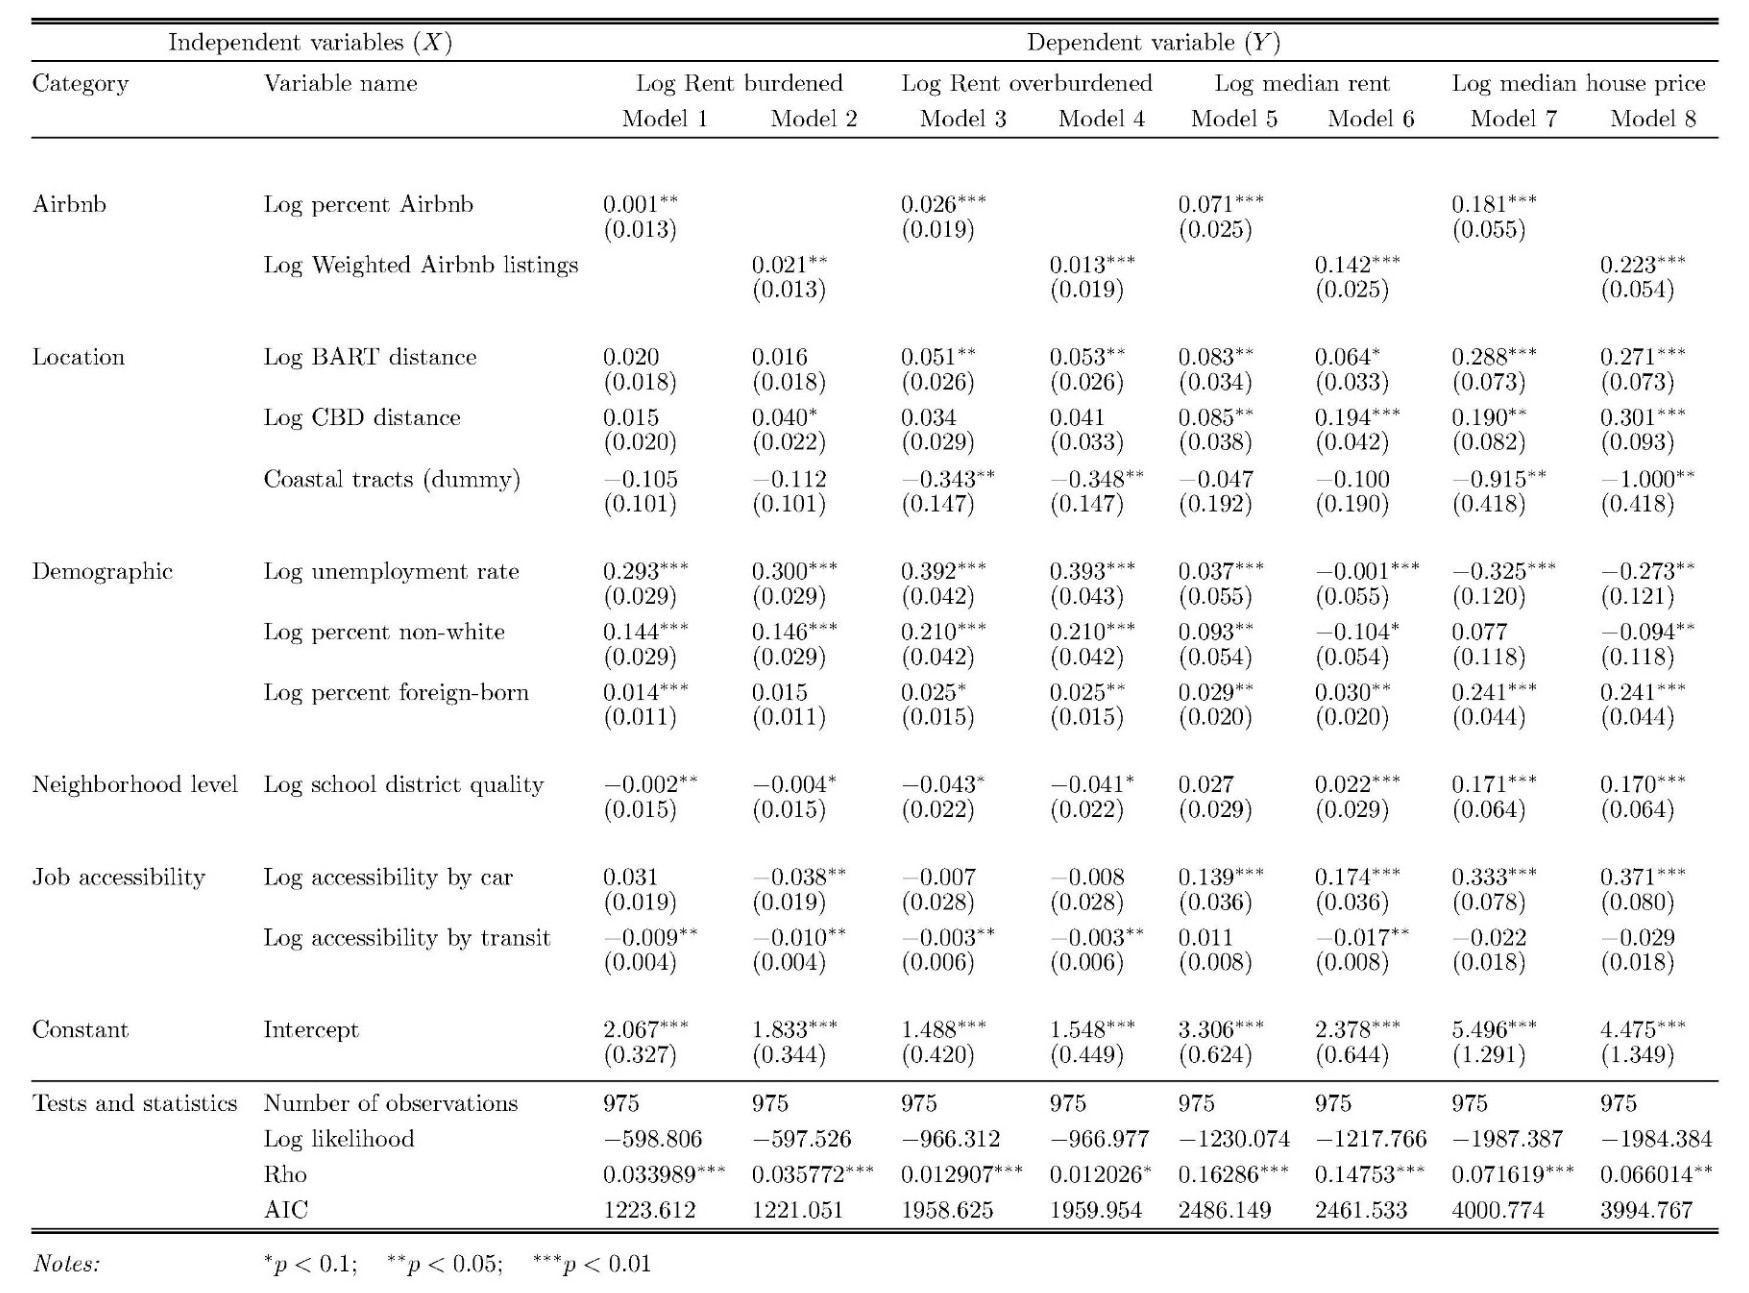
\includegraphics[width=1.1\textwidth]{table1}
  \caption{Coefficients and standard errors for Spatial Lag models}
\end{table}

Following observations can be made from the results of the spatial lag
model. To interpret the models, we pay attention to Probability values
(should be \(p<0.1\) for a significant correlation), Coefficient
values to ascertain the dependence of independent variable on \(Y\).

\begin{itemize}
\item
Both Airbnb variables (percent and weighted listings) have positive
coefficient for all eight models. Additionally, they are all
statistically significant.
\item
Location variables, \texttt{log BART dist.}\ and \texttt{log CBD dist.}\ show a positive
coefficient. This is as expected since proximity to BART stations and
downtown/central business districts is usually accompanied by higher
rents, house prices and hence more number of rent burdened and
overburdened households. The dummy location variable accounting for
whether or not a census tract is on the coast shows negative
coefficients for models 1, 2, 3 and 4 as expected. This can be
attributed to the fact that housing in coastal tracts (with views)
usually is premium housing and therefore attract only higher income
groups leading to lower rent burdened households. However, models 5, 6
7 and 8 either show statistically insignificant results or
counter-intuitive signs (negative). This indicates an opportunity to
use more nuanced variables representing coastal locations in the
study.
\item
All the demographic and neighborhood level variables show significant
correlation and similarly show expected signs.
\item
The job accessibility variables show mixed results. While most of the
coefficients are significant, it is hard to intuitively grasp the
reason behind their signs without resorting to more detailed
accessibility models.
\end{itemize}

The tests and statistics give the log likelihood and Akaike Information
Criteria results. Both these statistics indicate the quality of models.
A lower value of log likelihood and a larger value of AIC indicate a
better-quality model. Additionally, Rho statistic is significant for all
models and indicates high spatial dependence within the dataset. All the
models with percent Airbnb as the independent variables show better test
values than the weighted listings variables. Hence the results from
these models are further simulated below for more intuitive
understanding.

\begin{figure}
  \centering
  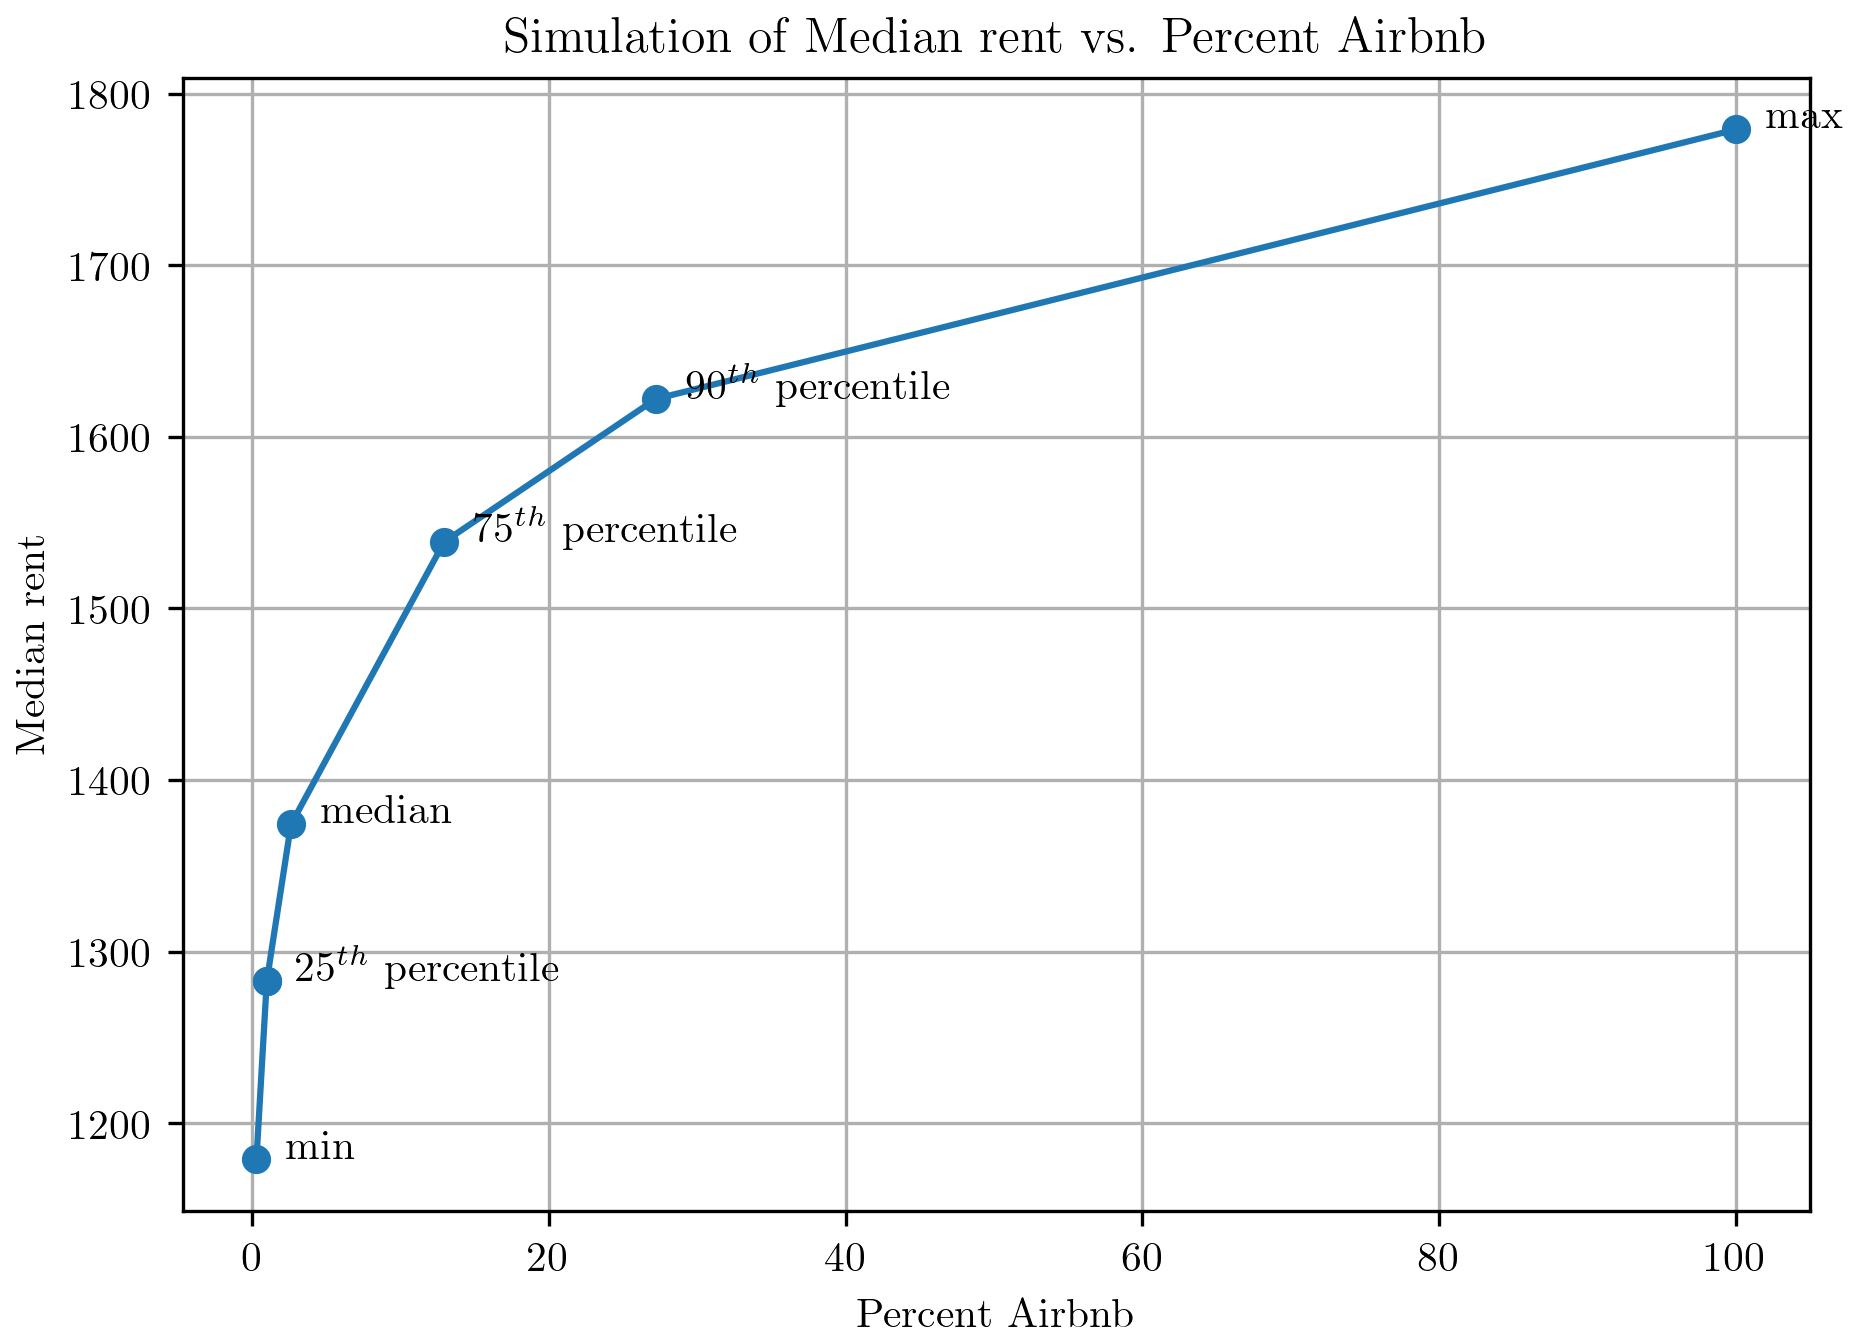
\includegraphics[width=0.49\textwidth]{Median_rent_vs_Percent_Airbnb.png}
  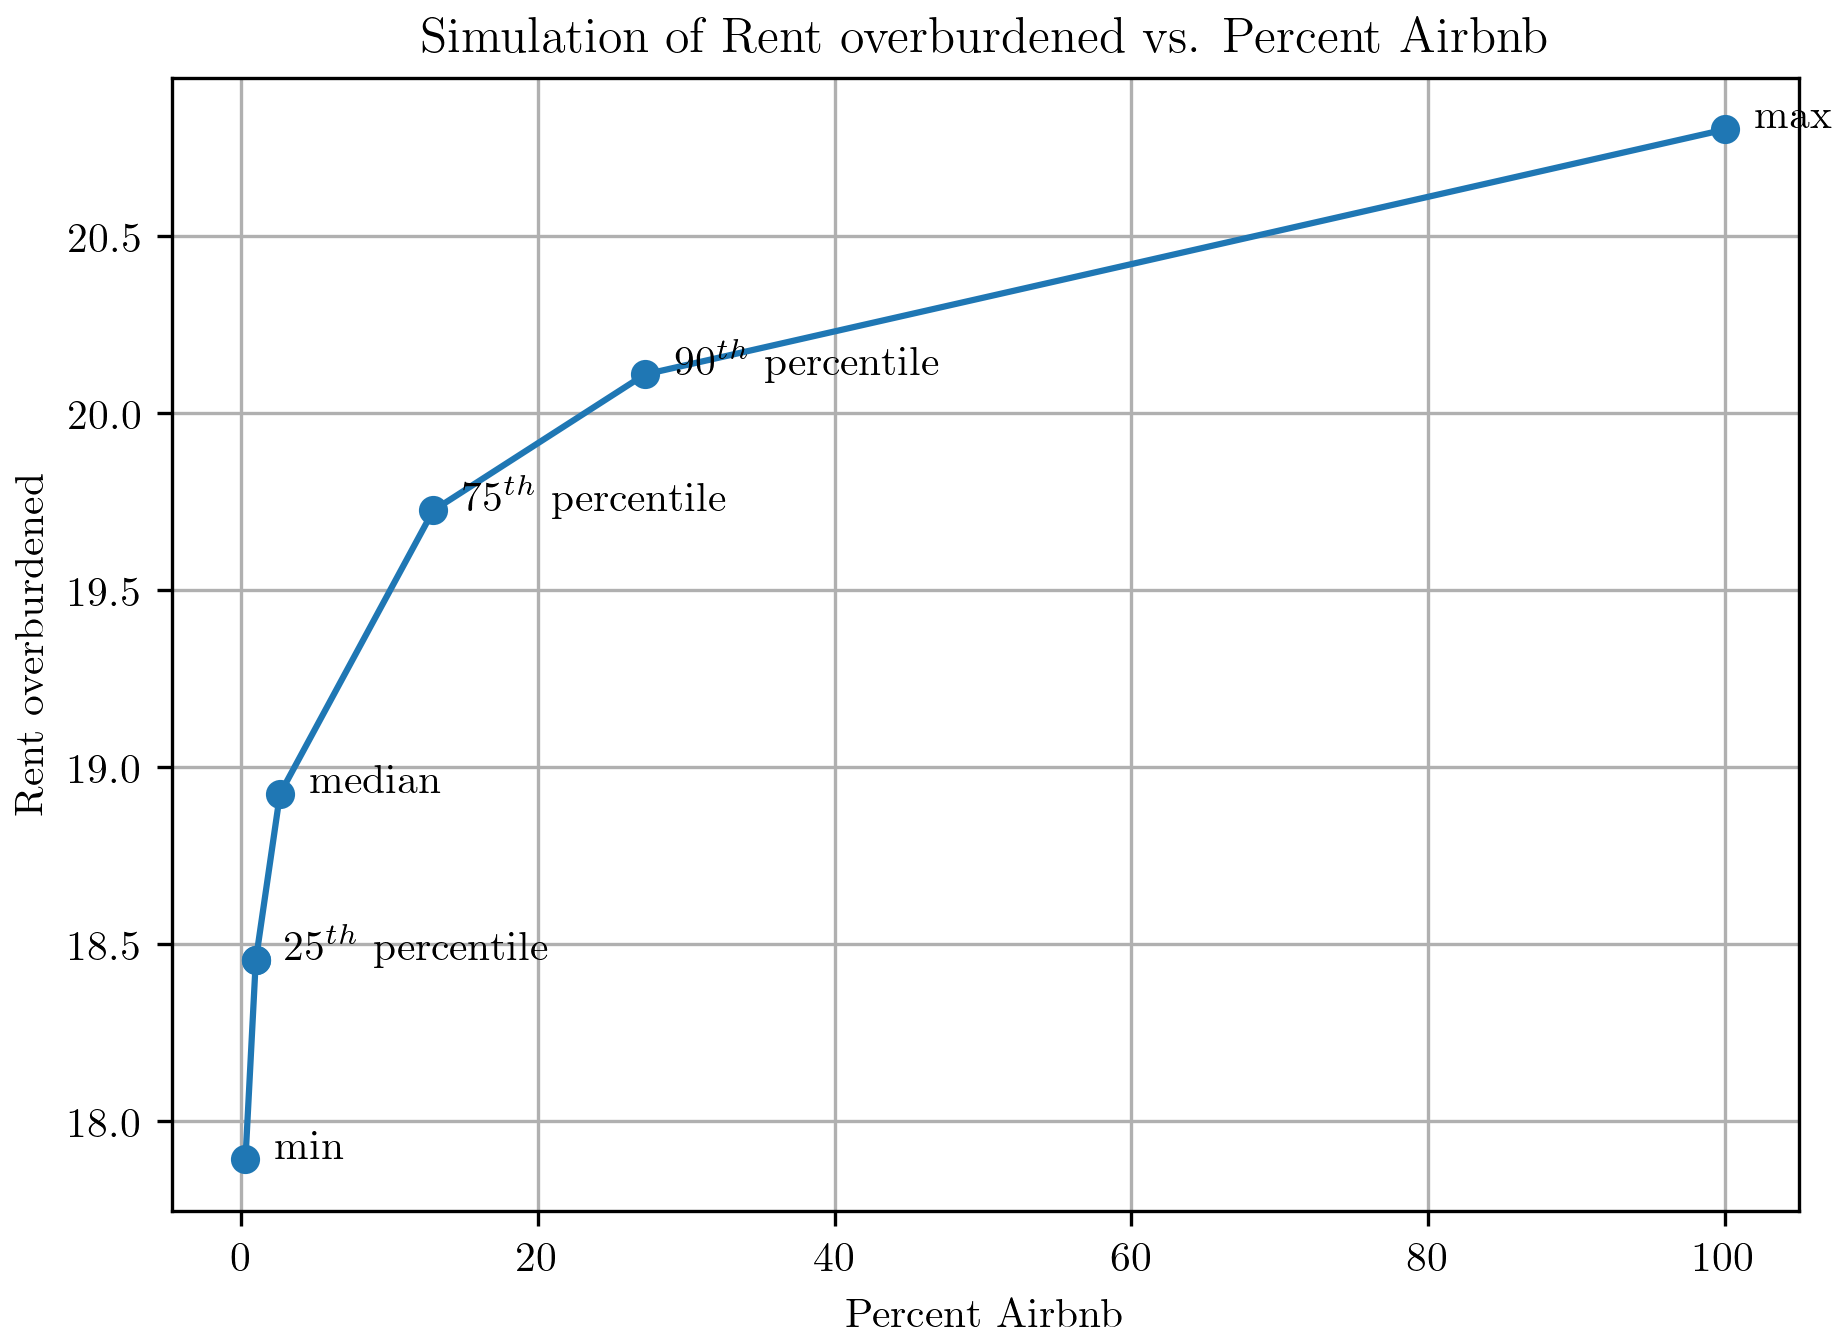
\includegraphics[width=0.49\textwidth]{Rent_overburdened_vs_Percent_Airbnb.png}
  \caption{Simulations for the cross-sectional analysis}
\end{figure}

Since both the independent and dependent variables were log-transformed
and fairly low in magnitude, we simulate the results by plotting values
estimated by the model at the \(0^\text{th}\) (min), \(25^\text{th}\), \(50^\text{th}\) (median), \(75^\text{th}\), \(90^\text{th}\)
and \(100^\text{th}\) (max) percentile of the \(X\) variable. These simulations show
that for a typical census tract (one with median percentage of Airbnb
listings, as a fraction of the rental housing market) a 1\% increase in
percent Airbnb listings corresponded to a 0.06\% rise in the rent
overburdened household category. Hence, in the case of a census tract
with 10,000 households, a 10\% increase in percent Airbnb listings will
correspond to 60 more households being added to the rent overburdened
category. This effect is more pronounced for tracts with a lower number
of Airbnb listings (\(10^\text{th}\) or \(25^\text{th}\) percentile). This would mean that
tracts with no or low percentage Airbnb listings will see more
households being pushed to a rent burdened category, with similar rise
in Airbnb listings.

In the case of median rents, for a typical census tract, a 1\% increase
in percent Airbnb listings corresponded to a \$12 hike in median gross
rents. For census tracts with a lower presence of Airbnb (\(25^\text{th}\)
percentile or lower), this number got as high as \$100.

In addition to the cross-sectional study, a longitudinal analysis of
panel data was also conducted ({\color{red}but not included in this extract}).
It is important to note here that the study area
for this analysis is the San Francisco City and not the whole MSA.
Hence, the unit of analysis is a census tract and the panel data
accounts for a four-year period from 2013 to 2016.

\begin{itemize}
\item Both Airbnb variables (\texttt{percent all rentals} and \texttt{percent active (occupied) rental housing}) have positive coefficient for all eight
models. Additionally, they are all statistically significant.

\item Location variables like \texttt{log BART distance} and \texttt{log CBD distances} and the time effects variable \texttt{trend} in some case are not significant
and in others, don't show consistent and expected trends.

\item In the case of demographic variables, \texttt{percent bachelor's degree}, \texttt{percent unemployed} and \texttt{median household income} variables show
significant and expected signs. However, \texttt{percent foreign-born} variable
does not.
\item
The \(R^2\) values for model \(1\) and \(2\) are higher and therefore a larger part of the variation in the \(Y\) is explained by the
independent variables \(X\) in these models. The adjusted \(R^2\) values show equivalent results.
\end{itemize}

\begin{table}[h]
  \hspace*{-0.8cm}
  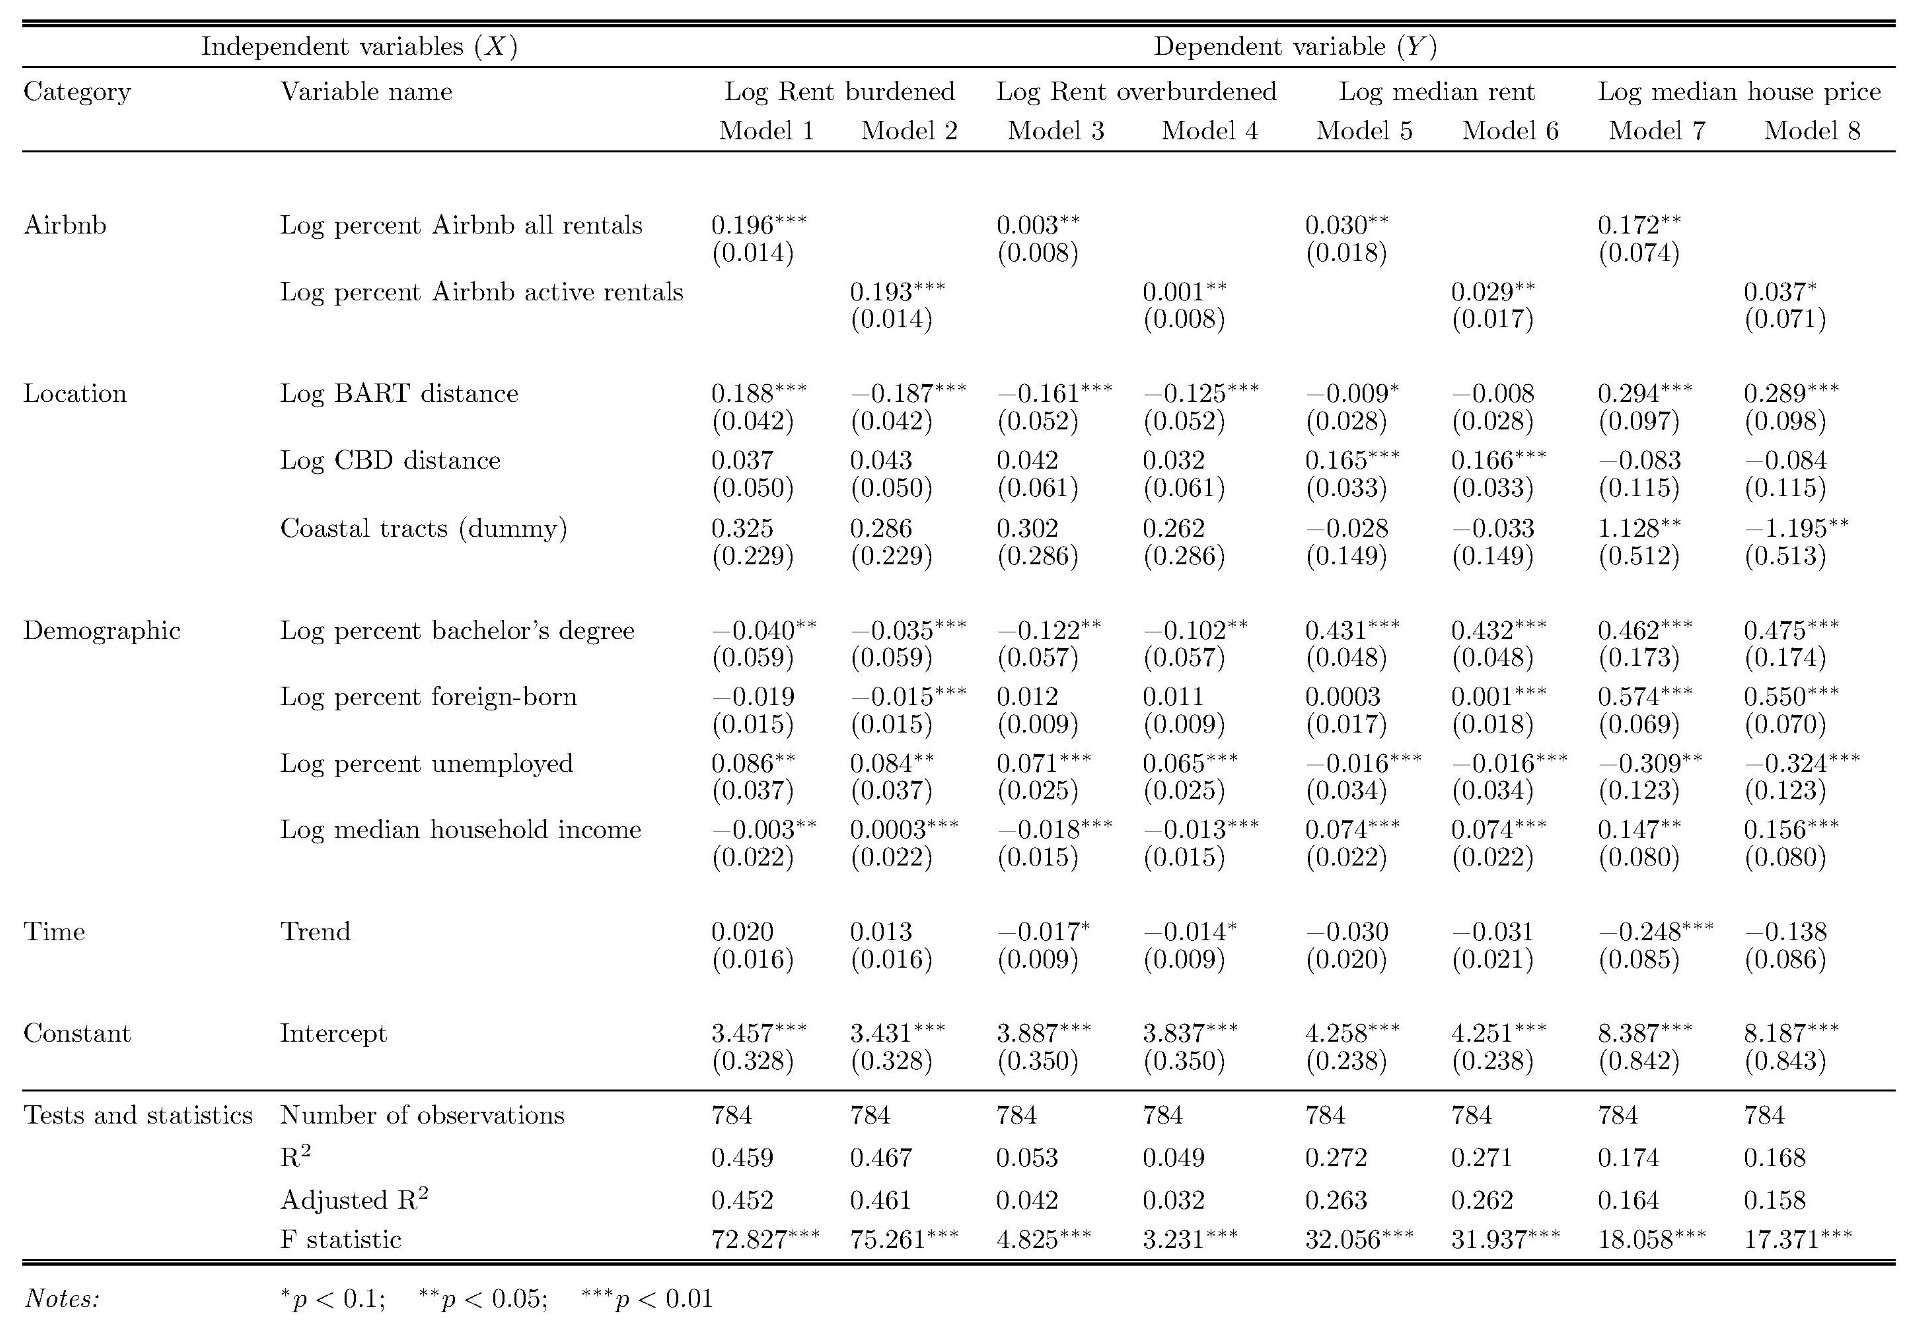
\includegraphics[width=1.1\textwidth]{table2.jpg}
  \caption{Coefficients and Standard errors for Random Effects Linear model}
\end{table}
\begin{figure}[H]
  \centering
  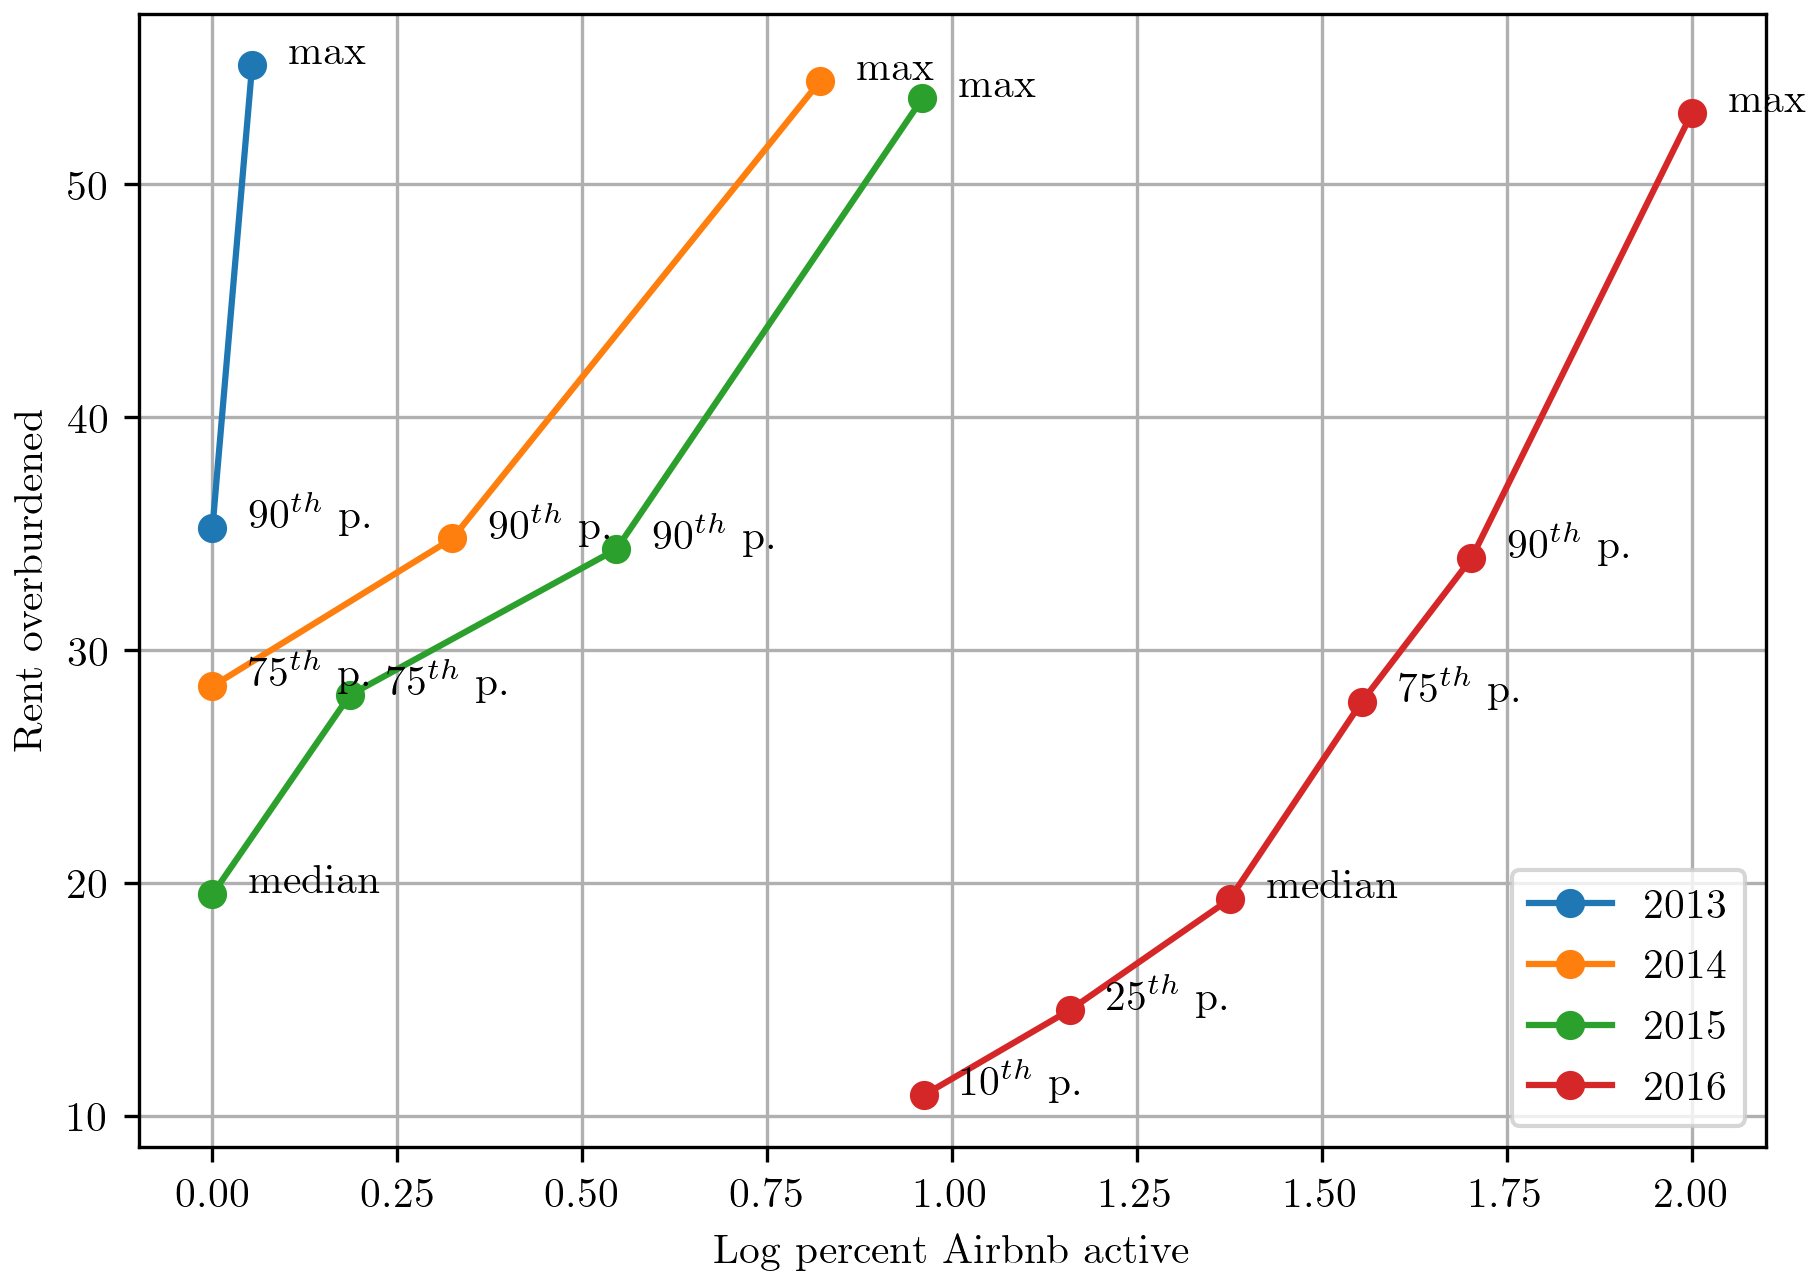
\includegraphics[width=0.7\textwidth]{Rent_overburdened_vs_Log_percent_Airbnb_active.png}
  \caption{Simulation of rent overburdened households vs.\ Airbnb listings for 2013--2016}
\end{figure}

Following observations can be made from the simulation of rent
overburdened households and percent Airbnb listings (as a fraction of
active/occupied rental units).

\begin{itemize}
\item Since both the independent and dependent variables were log-transformed and fairly-low in magnitude (coefficients), we
simulate the results by plotting values estimated by the model at the
\(10^\text{th}\), \(25^\text{th}\), \(50^\text{th}\) (median), \(75^\text{th}\), \(90^\text{th}\) and \(100^\text{th}\) (max) percentile of the
\(X\) variable.

\item Each simulation shows trends for \(Y\) vs.\ \(\log X\) for years 2013 to 2016.

\item Figure 6, overall trend shows that an increase in Airbnb active
rentals (Airbnb listings, as a fraction of occupied/active rental
housing market) corresponded to an increase in fractions of households
which were rent overburdened.

\item Furthermore, census tracts with a smaller presence of Airbnb listings
(those below 50th percentile) were more sensitive to an increase in
Airbnb listings i.e. they saw a higher increase in the
rent-overburdened household category as compared to census tracts in
the higher percentiles. This trend was consistent across all four
years.

\item A note of caution -- the \(x\)-axis for the simulation represents values
for log of the variable and care should be taken when reading off
numerical values from it.

\item Another way to read the simulation graph is to look at changes in rent
overburdened households for a fixed percentile mark across all four
years. Doing this for all percentiles (except the maximum), we observe
no significant change in the fraction of rent overburdened households
over the years.

\item The maximum value (\(100^\text{th}\) percentile) at first glance seems to be
decreasing over the years which is not the case.
However, these observations can be interpreted as an indication of a
trend wherein over the years, the census tracts with lower rent
overburdened populations have seen a larger increase in Airbnb
listings. This phenomenon results in a drop in the \(Y\) value associated
with the census tracts that have maximum percentage of listings which
is why the simulation for 2016 shows smaller values of \(Y\) as compared
to the other years. In effect, these values should not be compared
across the years without also accounting for shifting distributions of
Airbnb listings.
\end{itemize}

\begin{figure}[H]
  \centering
  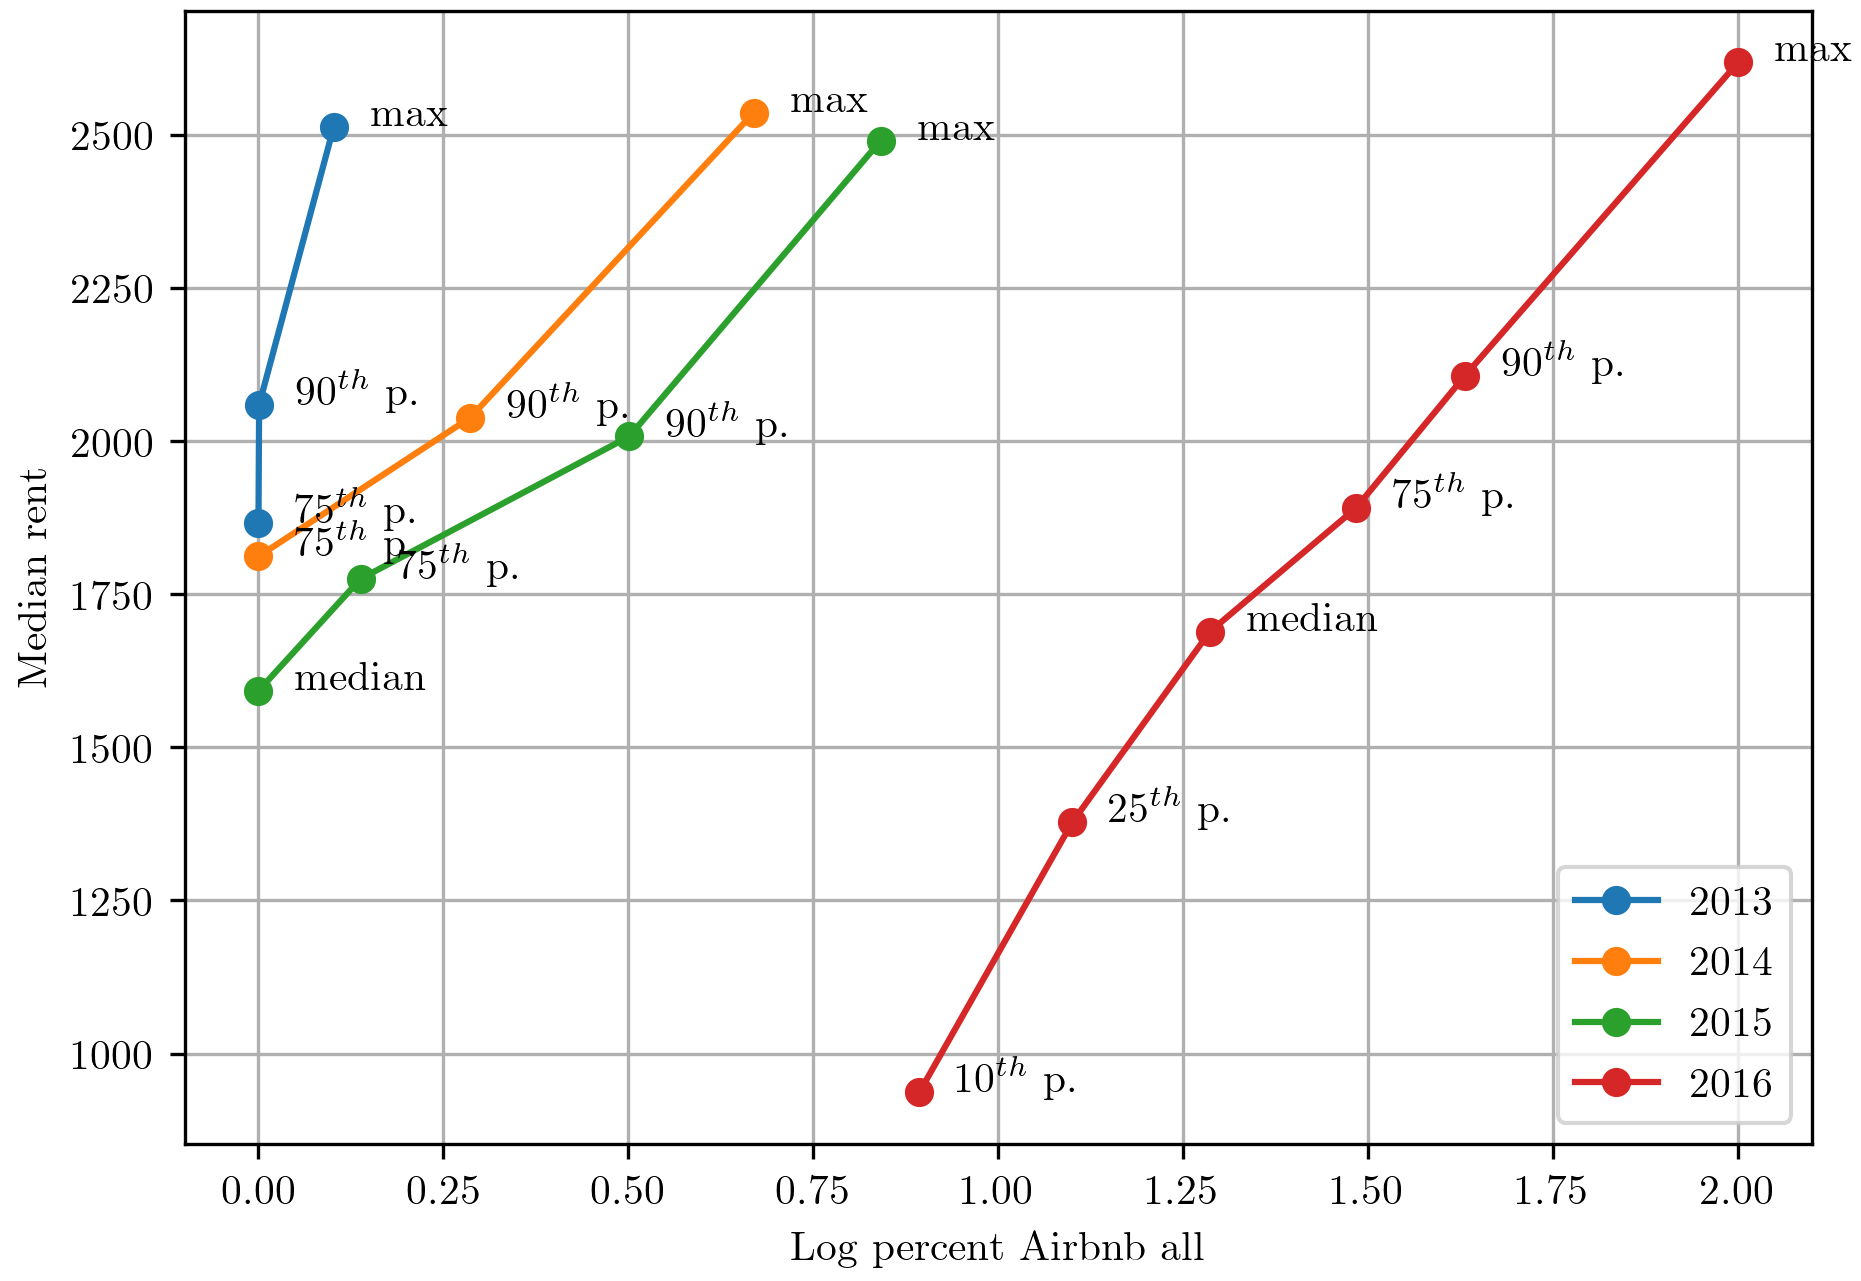
\includegraphics[width=0.7\textwidth]{Median_rent_vs_Log_percent_Airbnb_all.png}
  \caption{Simulation of median rent vs.\ Airbnb listings for 2013--2016}
\end{figure}

Following observations can be made from the simulation of median rents
and percent Airbnb listings (as a fraction of all rental units).

\begin{itemize}
\item
Figure 7, overall trend shows that an increase in Airbnb all rentals
(Airbnb listings, as a fraction of all rental housing in the market)
corresponded to an increase in the median rent per census tract.
\item
As before, for the early years (2013-14), we do not include data
points for the lower medians in the simulation in order to avoid
clustering of percentiles around zero. This is a consequence of fewer
tracts having Airbnb listings during that time.
\item
From the graph, we observe that census tracts with a smaller presence
of Airbnb listings (those below the \(50^\text{th}\) percentile) were more
sensitive to an increase in Airbnb listings i.e.\ they saw a higher
increase in the median rent per tract as compared to census tracts in
the higher percentiles. This trend was consistent across all four
years.
\item
A note of caution -- the \(x\)-axis for the simulation represents values
for log of the variable and care should be taken when reading off
numerical values from it.
\item
Another way to read the simulation graph is to look at changes in
median rent for a fixed percentile mark across all four years. Doing
this for all percentiles, we observe overall increases in the median
rent over the years for each of the \(50^\text{th}\) (median), \(75^\text{th}\), \(90^\text{th}\) and
\(100^\text{th}\) (maximum) percentiles.

\item Since both the \(y\)- and \(x\)-axes plot medians of the variables, one
should be extra-cautious while interpreting these results as they are
sensitive to the time-dependent probability distributions for these
variables.
\end{itemize}

\begin{figure}[H]
  \centering
  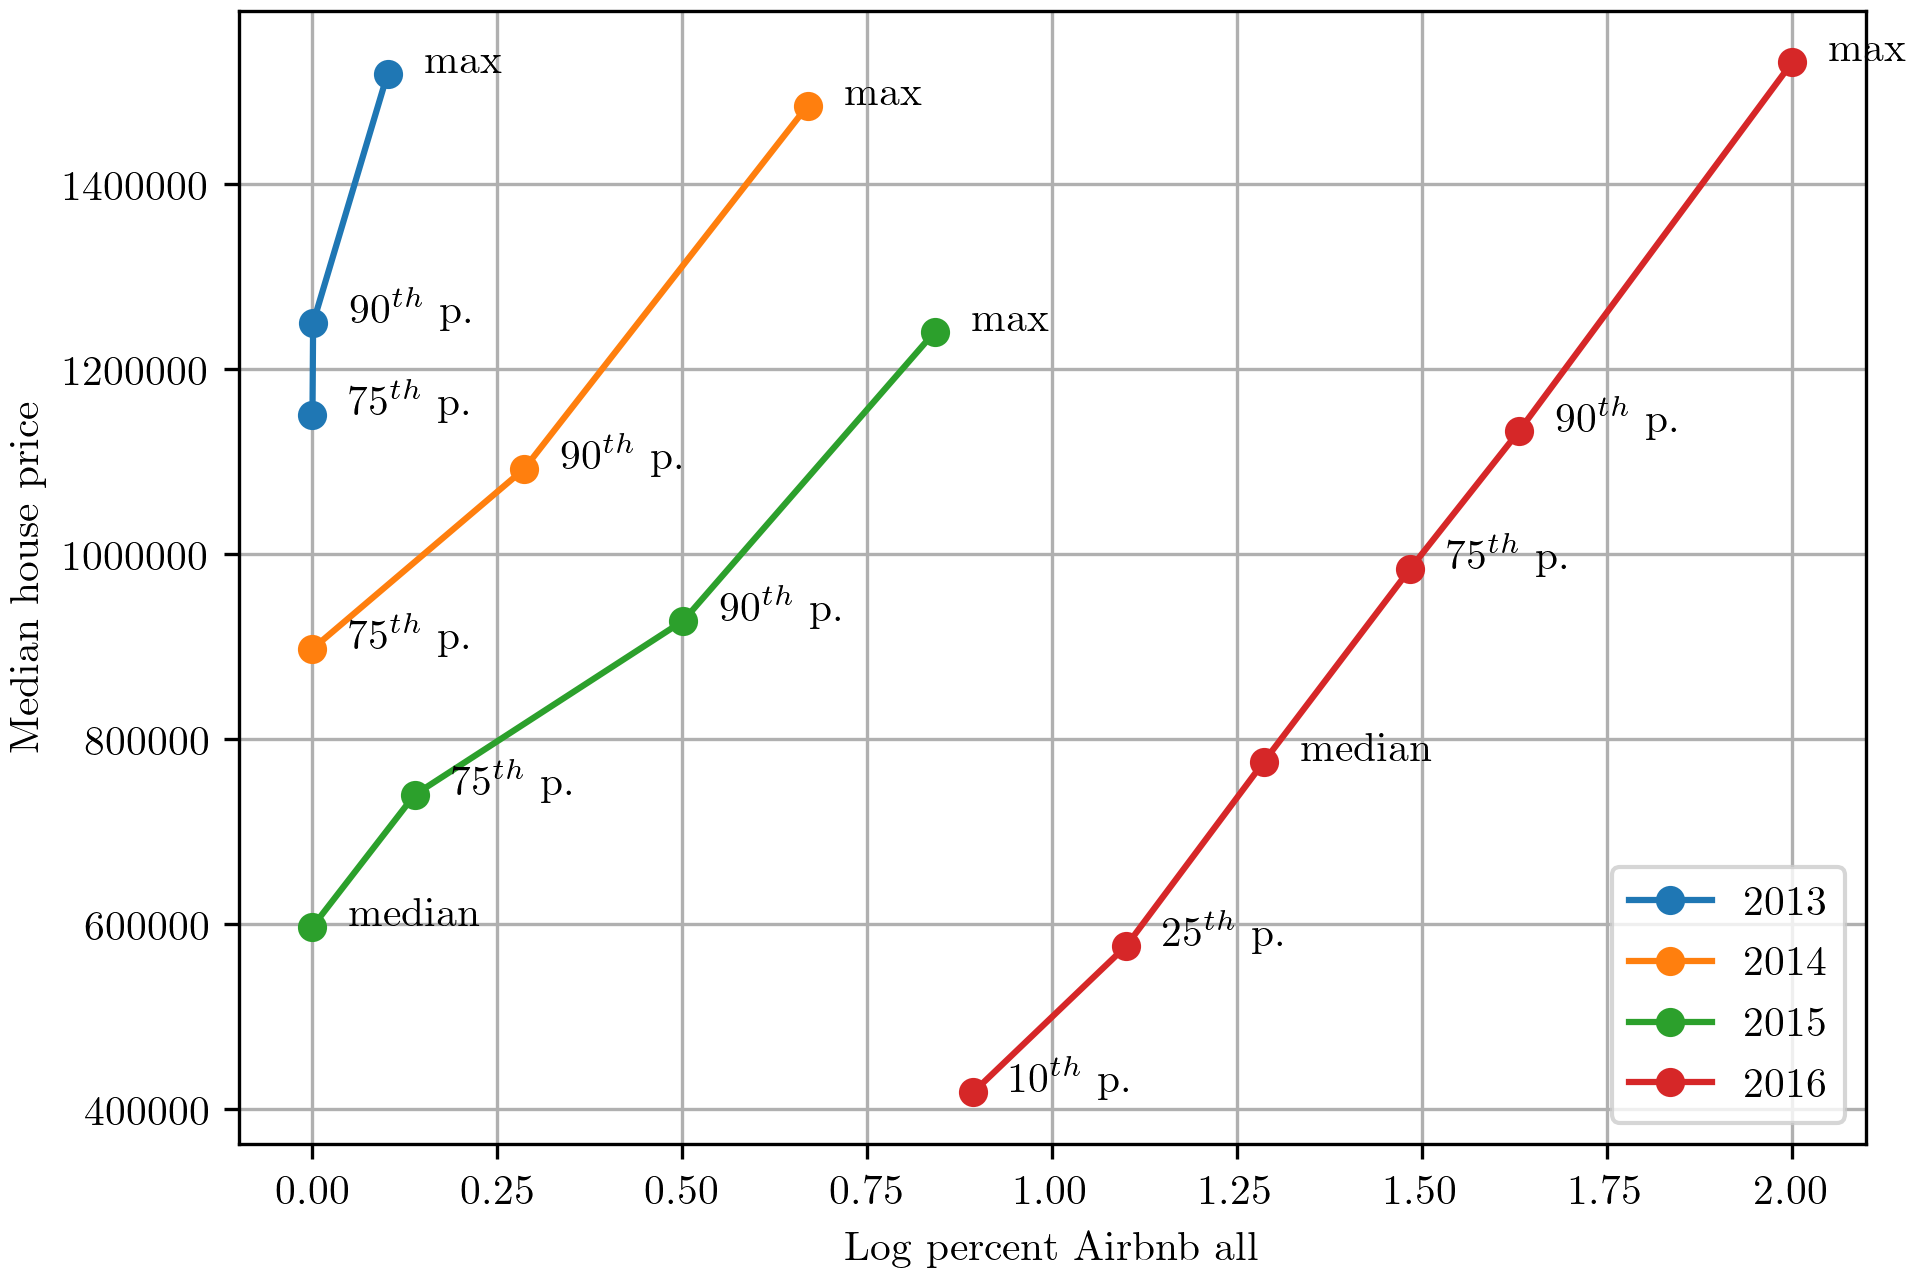
\includegraphics[width=0.7\textwidth]{Median_house_price_vs_Log_percent_Airbnb_all.png}
  \caption{Simulation of median house price vs Airbnb Listings for 2013--2016}
\end{figure}

Following observations can be made from the simulation of median house
prices and percent Airbnb listings (as a fraction of all rental units) ---

\begin{itemize}
\item Figure 8, the overall trend shows that an increase in Airbnb all
rentals (Airbnb listings, as a fraction of all rental housing in the
market) corresponded to an increase in the median house prices in
census tracts.
\item
As before, for the early years (2013--14), we do not include data
points for the lower medians in the simulation in order to avoid
clustering of percentiles around zero. This is a consequence of fewer
tracts having Airbnb listings during that time.
\item
From the graph, we observe that census tracts with a smaller presence
of Airbnb listings (those below the \(50^\text{th}\) percentile) were more
sensitive to an increase in Airbnb listings i.e.\ they saw a higher
increase in the median house price per tract as compared to census
tracts in the higher percentiles. This trend was consistent across all
four years.
\item
A note of caution -- the \(x\)-axis for the simulation represents values
for log of the variable and care should be taken when reading off
numerical values from it.
\item
Another way to read the simulation graph is to look at changes in
median house price for a fixed percentile mark across all four years.
Doing this for all percentiles, we observe a sharp and unexpected
decrease in the median house price (corresponding to these
percentiles) from 2013--2015. This does not mean that house prices were
decreasing in any way.
\item These observations can be interpreted as an indication of a trend
wherein over the years, the census tracts with lower house prices have
seen a larger increase in Airbnb listings. This phenomenon results in
a drop in the \(Y\) value for each of these percentiles which is why the
simulation for 2013--15 shows a decreasing trend in \(Y\). In effect, these
values should not be compared across the years without also accounting
for the time-dependent probability distributions for these variables
since both the \(y\)- and \(x\)-axes plot percentiles of the variables.
\end{itemize}


\section*{Chapter 5: Discussion and Conclusion}\label{sec: discussion-and-conclusion}

Using spatial regression analyses of cross-sectional and longitudinal
data specifically focusing on census tract level location, demographic,
neighborhood level, job accessibility and the main -- Airbnb variables
across the San Francisco MSA and the SF Francisco city, we aimed to
address the following: Do short-term rentals in the form of Airbnb
rentals impact the rent affordability of the study area and if so then
to what extent? Overall, we find a significant correlation between the
indicators Airbnb's presence (percent Airbnb listings as a fraction of
total rental housing available and weighted Airbnb listings) and various
rental affordability measures (rent-burdened households, rent
overburdened households, median rents, and median house prices). While
the correlation does not mean causation, the relative magnitudes of
coefficients can be simulated for better understanding. The simulations
from the spatial lag models (cross-sectional study) provide useful
insights about the relationship between Airbnb and rental affordability.
These also reveal that the tracts with lower percentages of Airbnb
listings are more at risk of having low rental affordability as the
presence of Airbnb increases.

This research also finds its motivation in connecting its findings with
the regulatory debate. While a more comprehensive and deeper analysis is
warranted for estimating a regulatory response (if any) to the platform,
it is important to ascertain its effects both positive and negative. One
critical dissection that should be acknowledged is that of the casual
and commercial hosts. While the casual hosts stay true to the spirit of
home-sharing i.e.\ utilization of underutilized/latent resources to
support their incomes, the billion-dollar company seems to find its
major revenue source in the commercial hosts (sometimes the super hosts)
who own multiple properties and have entire house listings available
throughout the year. Such hosts could have been landlords as part of the
long-term rental housing stock. In a bid to investigate the revenue
potential of Airbnb hosts as opposed to becoming a landlord in the same
area, one can compare certain numbers available. While this analysis is
not extensive, the main purpose of it is to understand how lucrative it
is for the hosts to rent with Airbnb, rather than putting their property
for long-term renting. The data shown is collected from AirDNA, (a paid
service that provides Airbnb data analytics) mainly created to assist
hosts to decide on their listing prices and better understand revenue
trends. This study used the free data points that are available on the
website i.e. county-wise average revenue earned by Airbnb hosts monthly
(for 2017). The vacancy rates assumed for these estimates were not
disclosed by the service. These revenue amounts can be compared with the
gross median rent in that county to understand the difference between
renting for long term vs short term. Table 5 shows the difference
between renting with Airbnb (short-term) and renting lease based for
long-term.

\begin{table}[H]
  \footnotesize
  \centering
  \def\arraystretch{1.1}
  \begin{tabular}{lllll}
    \toprule
    \textbf{County}        & \textbf{Avg.\ monthly} & \textbf{Median gross} & \textbf{Ratio}          & \textbf{Percent entire}\\
            & \textbf{revenue}       & \textbf{rent}         & \textbf{(revenue/rent)} & \textbf{home listings}\\
    \midrule
    San Francisco & \$ 3,107      & \$ 1,784          & 1.74                 & 59\%\\
    Alameda       & \$ 2,155      & \$ 1,622          & 1.33                 & 59\%\\
    San Mateo     & \$ 2,375      & \$ 2,114          & 1.12                 & 42\%\\
    Marin         & \$ 2,298      & \$ 1,921          & 1.20                 & 60\%\\
    Contra Costa  & \$ 1,466      & \$ 1,692          & 0.87                 & 37\%\\
    \bottomrule
  \end{tabular}
\caption{Comparison of revenue earned as an Airbnb host to that earned as landlord.}
\end{table}

It can be observed that except Contra Costa County, all other counties
present lucrative options for the Airbnb hosts to rent short-term
instead of long-term. However, it should also be noted that the highest
earning hosts are the commercial or the super hosts who host multiple
entire home listings. Hence, an important consideration for regulating
Airbnb and like platforms are targeted policies ensuring proliferation
of casual hosts who make tourism more affordable, benefit local business
and empower homeowners by providing extra income but keeping a check on
the commercial hosts who can potentially skirt hotel taxes and
regulations by participating in the `sharing' economy model. This
presents as an opportunity for planners to evaluate their policies and
development controls to better respond to Airbnb and the sharing
economy. These can include better zoning provisions, extensive research
and analysis of neighborhoods with high Airbnb listing concentrations,
keeping an eye out for gentrification indicators and affordability
concerns etc. Incentives can be promoted for the casual hosts who in way
stay true to the idea of sharing economy. One major challenge in this
process is to establish data sharing between Airbnb and planning
agencies to better gauge the impacts and extent of the model. This
leaves a lot of scope for research in terms of assessing neighborhood
level impacts, negative and positive externalities of increase in Airbnb
listings in a certain area and the need and type of regulation needed to
accommodate Airbnb and sharing economy in general.

\section*{References}

\begin{enumerate}
\item Anselin, L. (2017), \emph{Spatial Data Science}. [Video file] Retrieved from
\\\texttt{www.youtube.com/channel/UCzvhOfSmJpRsFRF2Pgrv-Wg}

\item Aurand, A. (2016). Out of Reach 2016: No Refuge for Low Income Renters.
\emph{National Low-Income Housing Coalition.} Retrieved from: \texttt{http://nlihc.org/sites/default/files/oor/OOR\_2016.pdf}

\item Barron, K., Kung, E. and Proserpio, D. (2018) \emph{The Sharing Economy and Housing Affordability: Evidence from Airbnb.} Retrieved from SSRN:
  \texttt{https://ssrn.com/abstract=3006832}

\item Budget and legislative analyst (2016) Policy Analysis Report, Board of Supervisors, \emph{City and County of San Francisco.} Retrieved from:
  \\\texttt{https://sfbos.org/sites/default/files/FileCenter/Documents/}
  \\\hspace*{1cm}\texttt{55575-BLA.ShortTermRentals\%20040716.pdf}

\item Bensinger, G. (2017) Airbnb Valued at \$31 Billion After New Funding Round; Home-sharing site adds \$1 billion cash cushion to stave off IPO, \emph{Wall Street
    Journal} (Online); New York, N.Y. \mbox{Retrieved} from:
  \\\texttt{https://www.wsj.com/articles/}
  \\\hspace*{1cm}\texttt{airbnb-valued-at-31-billion-after-new-funding-round-1489086240}

\item Codagnone, C. and Martens, B. (2016). Scoping the Sharing Economy: Origins, Definitions, Impact and Regulatory Issues. \emph{Institute for
    Prospective Technological Studies Digital Economy Working Paper 2016/01}. DOI: JRC100369

\item Codagnone, C., Biagi, F., and Abadie, F. : The Passions and the Interests: Unpacking the 'Sharing Economy'. \emph{Institute for Prospective
    Technological Studies, JRC Science for Policy Report EUR 27914 EN,} DOI:10.2791/474555

\item Gutierrez, J., Garcia, J., Romanillos, G. and Olmedo. M. (2016). The eruption of airbnb in tourist cities: comparing spatial patterns of
hotels and peer-to-peer accommodation. \emph{Tourirm Management, Elsevier Ltd}. Retrieved from:
\\\texttt{http://isiarticles.com/bundles/Article/pre/pdf/148944.pdf}

\item Guttentag, D.\ (2015).\ Airbnb: disruptive innovation and the rise of an informal tourism accommodation sector. \emph{Current Issues in Tourism}, 10(12), 1192-1217.

\item Hooijer, P. (2016). The Relationship between Airbnb and the Hotel Revenue: Evidence from The Netherlands. \emph{University of Amsterdam.} Retrieved from:
  \\\texttt{http://www.scriptiesonline.uba.uva.nl/608470}

\item Kaplan, R. A. (2015). Airbnb: A Case Study in Occupancy Regulation and
Taxation. \emph{The University of Chicago Law Review Dialogue}, p103-115.

\item Lee, D. (2015). How Airbnb Short-Term Rentals Exacerbate Los Angeles's
Affordable Housing Crisis: Analysis and Policy Recommendations. 10, 229-253.

\item Malhotra, A., and Van Alstyne, M. (2014). The dark side of the sharing
economy and how to lighten it. \emph{Communications of the ACM}, 57, 24-27.

\item Meni, D. (2017, March 21). Are Airbnbs driving up your rent? Retrieved
from:
\\\texttt{https://ggwash.org/view/62774/are-airbnbs-driving-up-your-rent}

\item Gurran, N. and Phibbs, P. (2017) When Tourists Move In: How Should Urban
Planners Respond to Airbnb?, \emph{Journal of the American Planning Association,}
83:1, 80-92,\\DOI: 10.1080/01944363.2016.1249011

\item O'Sullivan, F. (2015, December 23). Tourist-Heavy Barcelona Is Cracking
Down on Airbnb. Retrieved from:
\\\texttt{https://www.citylab.com/equity/2015/12/barcelona-airbnb-tourism/421788/}

\item PricewaterhouseCoopers (PwC) report. (2014). The sharing economy: How will it disrupt your business? Retrieved from --
\\\texttt{http://www.pwc.co.uk/economic-policy/index.jhtml}

\item Quattrone, G., Proserpio, D., Quercia, D., Capra, L., and Musolesi, M. (2016). Who Benefits from the ``Sharing'' Economy of Airbnb? \emph{Cornel University Library} Retrieved from: 
\\\texttt{https://arxiv.org/pdf/1602.02238}

\item Shaheen, S., Sperling, D., and Wagner, C. (1999). A Short History of Carsharing in the 90's.\emph{Journal of World Transport Policy and Practice}, 5(3), 18-40.

\item Shephard, S. and Udell, A. (2016). Do Airbnb properties affect house prices? \emph{New York State Office of the Attorney General,} supra note 42 at
  2, 10-11. Retrieved from: 
\\\texttt{https://ag.ny.gov/pdfs/AIRBNB\%20REPORT.pdf}

\item Streitfeld, D. (2014, October 15). Airbnb Listings Mostly Illegal\emph{,} New York State Contends. \emph{New York Times.}
Retrieved from:
\\\texttt{https://www.nytimes.com/2014/10/16/business/}
\\\hspace*{1cm}\texttt{airbnb-listings-mostly-illegal-state-contends.html}

\item Stulberg, A. (2016). Airbnb Probably Isn't Driving Rents Up Much, At Least Not Yet. Retrieved from:
\\\texttt{https://fivethirtyeight.com/features/}
\\\hspace*{1cm}\texttt{airbnb-probably-isnt-driving-rents-up-much-at-least-not-yet/}

\item Zervas, G., Byers, J. and Proserpio, D. (2016). The Rise of the Sharing Economy: Estimating the Impact of Airbnb on the Hotel Industry.
Retrieved from: 
\\\texttt{http://people.bu.edu/zg/publications/airbnb.pdf}
\end{enumerate}

\end{document}